\documentclass[a0paper,portrait]{baposter}
\usepackage{comment}
\usepackage{multicol}
\usepackage{wrapfig}
\usepackage{lmodern}
\usepackage{lipsum,graphicx}
\usepackage{multirow}
\usepackage[utf8]{inputenc} %unicode support
\usepackage[T1]{fontenc}
\usepackage{enumitem}
\usepackage{setspace}

\selectcolormodel{cmyk}

\graphicspath{{pics/}} % Directory in which figures are stored

\newcommand{\compresslist}{%
\setlength{\itemsep}{0pt}%
\setlength{\parskip}{1pt}%
\setlength{\parsep}{0pt}%
}

\newenvironment{boenumerate}
  {\begin{enumerate}\renewcommand\labelenumi{\textbf\theenumi.}}
  {\end{enumerate}}


\begin{document}

\definecolor{Mycolor1}{HTML}{222222}
\definecolor{Mycolor2}{HTML}{FFFF00}
\definecolor{graz_yellow}{HTML}{FFDF00}
\definecolor{graz_gray}{HTML}{666666}
\definecolor{graz_black}{HTML}{000000}

\begin{poster}
{
grid=false,
headerborder=open, % Adds a border around the header of content boxes
colspacing=1em, % Column spacing
bgColorOne=white, % Background color for the gradient on the left side of the poster
bgColorTwo=white, % Background color for the gradient on the right side of the poster
borderColor=Mycolor1, % Border color
headerColorOne=graz_yellow, % Background color for the header in the content boxes (left side)
headerColorTwo=graz_black, % Background color for the header in the content boxes (right side)
headerFontColor=graz_black, % Text color for the header text in the content boxes
boxColorOne=white, % Background color of the content boxes
textborder=faded, %rectangle, % Format of the border around content boxes, can be: none, bars, coils, triangles, rectangle, rounded, roundedsmall, roundedright or faded
eyecatcher=false, % Set to false for ignoring the left logo in the title and move the title left
headerheight=0.11\textheight, % Height of the header
headershape=rectangle, % Specify the rounded corner in the content box headers, can be: rectangle, small-rounded, roundedright, roundedleft or rounded
headershade=plain,
headerfont=\Large\textsf, % Large, bold and sans serif font in the headers of content boxes
%textfont={\setlength{\parindent}{1.5em}}, % Uncomment for paragraph indentation
linewidth=2pt % Width of the border lines around content boxes
}

%
%%% Title %%%%%%%%%%%%%%%%%%%%%%%%%%%%%%%%%%%%%%%%%%%%%%%%%%%%%%%%%%%%%%%%%%%%%
{
\textsf{Robust Textline Annotation and Extraction\\ for HTR on Medieval Charters}
}
%%% Authors %%%%%%%%%%%%%%%%%%%%%%%%%%%%%%%%%%%%%%%%%%%%%%%%%%%%%%%%%%%%%%%%%%%
{
\sf\vspace{.2em}\\
A. Uthor, C. Ontributor
\vspace{.2em}\\
{\small Department of Digital Humanities, University of Graz}
}
% For contributors from different labs:
% {
% \sf\vspace{.2em}\\
% A. Uthor$^{1}$, C. Ontributor$^{2}$
% \vspace{.2em}\\
% $^{1}$Department of Digital Humanities, University of Graz\\
% $^{2}$Institute for Machine Learning, TU Graz
% }
{

\includegraphics[width=.17\linewidth]{unigraz_logo.png} % UniGraz logo
}

% this states the box starts at column 0 (edge of page), row 0 (top of page) for a span of 3 (columns wide)
\headerbox{Introduction}{name=introduction,column=0,row=0, span=3}{
	\small
    \lipsum*[19]
	\vspace{1em}

	%\setlist{nolistsep} % makes space above the list tighter
    \begin{minipage}{.48\linewidth}
		\textbf{Challenges:}
		\begin{itemize}
            \compresslist % more compact list items
			\item Ex sapien vitae pellentesque sem placerat in id.
			\item Pretium tellus duis convallis tempus leo eu aenean.
		\end{itemize}
	\end{minipage}%
	\hfill\vline\hfill%
	\begin{minipage}{.48\linewidth}
		\textbf{Constraints:}
		\begin{itemize}
            \compresslist
			\item Montes nascetur ridiculus mus donec rhoncus eros lobortis.
            \item Aenean sed diam urna tempor pulvinar vivamus fringilla. 
			\end{itemize}
	\end{minipage}
}
\newcommand{\compresslist}{
	\setlength{\itemsep}{1pt}
	\setlength{\parskip}{0pt}
	\setlength{\parsep}{0pt}
}


% this states the box starts at column 0 (edge of page), directly below the box labelled 'corpus' for a span of 1 (column wide)
\headerbox{Figures}{name=corpus,column=0,below=introduction,span=1}{

	\small
	    
        \begin{minipage}{\textwidth}
        \centering
        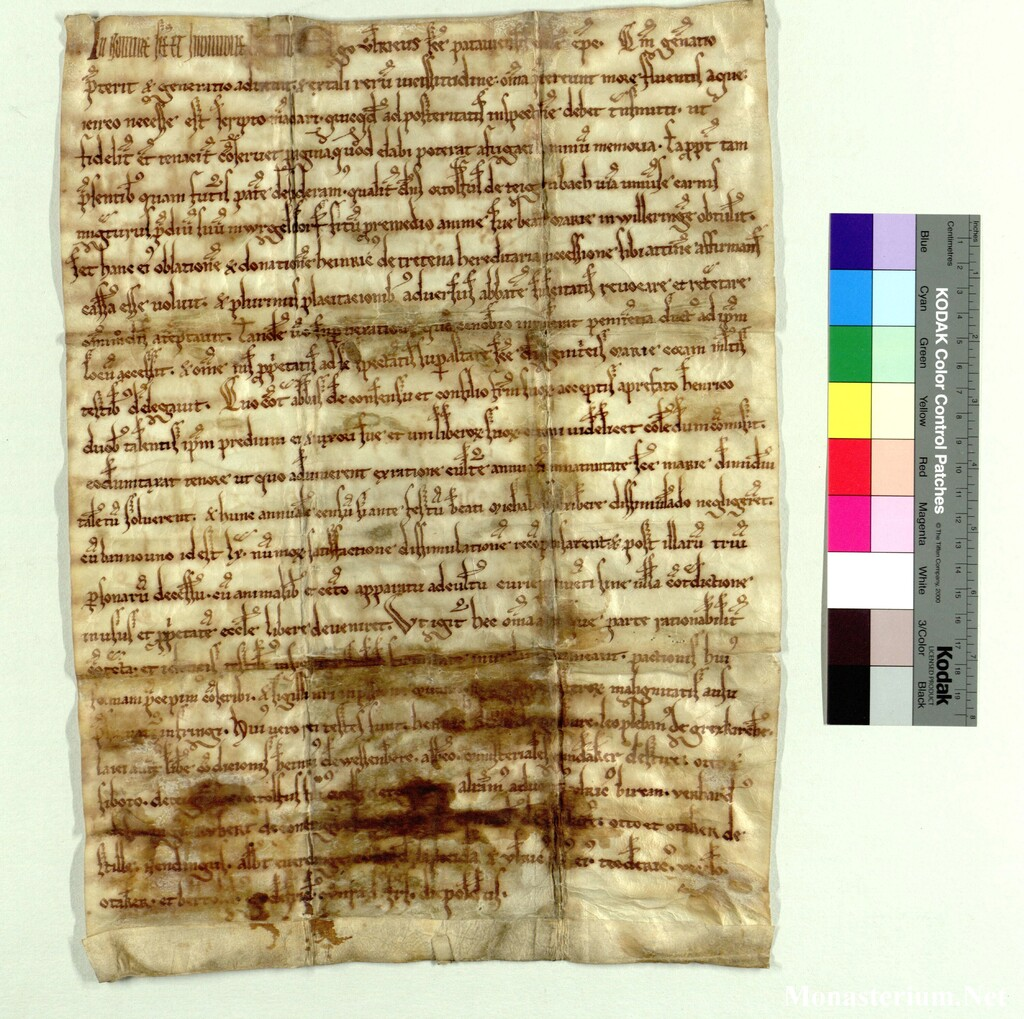
\includegraphics[width=.6\textwidth]{9bde06a84833576b4027ae6331553753.img.jpg}\\
         \vspace{.1em}
         Fig.~1: A charter
        \end{minipage}
        \vspace{1em}
        
        \lipsum*[2][1-5]
}

\headerbox{Paragraph with wrapped figure}{name=subcorpus,column=1,below=introduction,span=1}{
\lipsum[10]
}

\headerbox{Vertical span}{name=vertical,column=2,below=introduction,height=2}{
\lipsum[10]
}



\headerbox{Compressed lists}{name=segmentation,column=0,span=2,below=corpus}{

\begin{center}
\includegraphics[width=.85\linewidth]{pics/segmentation_pipeline.pdf}
\end{center}
\footnotesize
\begin{multicols}{2}
	A list:
	\begin{itemize}
        \compresslist
		\item Etiam volutpat sem sed felis pulvinar consequat.
		\item In lobortis mi nec nulla dictum, sed interdum sapien scelerisque.
		\item Nam non nulla at lectus rhoncus lacinia.
	\end{itemize}
    \lipsum[1]
\end{multicols}

}

\headerbox{Fusce Feugiat Rutrum Magna}{name=htr,column=0,below=segmentation,span=2,above=bottom}{



%	\begin{itemize}
%    \item{Nicolaou, A., Christlein, V., Riba, E., Shi, J., Vogeler, G., \& Seuret, M. (2022). TorMentor: Deterministic dynamic-path, data augmentations with fractals. In Proceedings of the IEEE/CVF Conference on Computer Vision and Pattern Recognition (pp. 2707–2711).    
%    }
%    \item{Nicolaou, A., Luger, D., Decker, F., Renet, N., Christlein, V., \& Vogeler, G. (2023). Efficient Annotation of Medieval Charters. arXiv preprint arXiv:2306.14071.    
%\end{itemize}
}


\headerbox{References}{name=references,column=2,below=segmentation,span=1,above=bottom, headerColorOne=white}{
\small
	Segmentation corpus (831 charters with JSON annotation): \texttt{https://zenodo.org/records/15460694}

\vspace{1em}
	Line annotation tool: 

	{\footnotesize \texttt{https://github.com/nicolasrenet/ch-lat.git}}
\vspace{1em}

	Line segmentation pipeline:
	
	{\footnotesize \texttt{https://github.com/nicolasrenet/ddpa\_lines\_ng.git}}
\begin{center}
\begin{tabular}{cc}

\includegraphics[width=1.8cm]{monasterium_qrcode.png} & 
\includegraphics[width=2.1cm]{pqr_didip.png} \\
	Monasterium & DiDip
\end{tabular}
\end{center}
}


\end{poster}

\end{document}
